%%%%%%%%%%%%%%%%%%%%%%%%%%%%%%%%%%%%%%%%%
% Beamer Presentation
% LaTeX Template
% Version 1.0 (10/11/12)
%
% This template has been downloaded from:
% http://www.LaTeXTemplates.com
%
% License:
% CC BY-NC-SA 3.0 (http://creativecommons.org/licenses/by-nc-sa/3.0/)
%
%%%%%%%%%%%%%%%%%%%%%%%%%%%%%%%%%%%%%%%%%

%----------------------------------------------------------------------------------------
%	PACKAGES AND THEMES
%----------------------------------------------------------------------------------------

\documentclass{beamer}

\mode<presentation> {

% The Beamer class comes with a number of default slide themes
% which change the colors and layouts of slides. Below this is a list
% of all the themes, uncomment each in turn to see what they look like.

%\usetheme{default}
%\usetheme{AnnArbor}
%\usetheme{Antibes}
%\usetheme{Bergen}
%\usetheme{Berkeley}
%\usetheme{Berlin}
%\usetheme{Boadilla}
%\usetheme{CambridgeUS}
%\usetheme{Copenhagen}
%\usetheme{Darmstadt}
%\usetheme{Dresden}
%\usetheme{Frankfurt}
%\usetheme{Goettingen}
%\usetheme{Hannover}
%\usetheme{Ilmenau}
%\usetheme{JuanLesPins}
%\usetheme{Luebeck}
\usetheme{Madrid}
%\usetheme{Malmoe}
%\usetheme{Marburg}
%\usetheme{Montpellier}
%\usetheme{PaloAlto}
%\usetheme{Pittsburgh}
%\usetheme{Rochester}
%\usetheme{Singapore}
%\usetheme{Szeged}
%\usetheme{Warsaw}

% As well as themes, the Beamer class has a number of color themes
% for any slide theme. Uncomment each of these in turn to see how it
% changes the colors of your current slide theme.

%\usecolortheme{albatross}
%\usecolortheme{beaver}
%\usecolortheme{beetle}
%\usecolortheme{crane}
%\usecolortheme{dolphin}
%\usecolortheme{dove}
%\usecolortheme{fly}
%\usecolortheme{lily}
%\usecolortheme{orchid}
%\usecolortheme{rose}
%\usecolortheme{seagull}
%\usecolortheme{seahorse}
%\usecolortheme{whale}
%\usecolortheme{wolverine}

%\setbeamertemplate{footline} % To remove the footer line in all slides uncomment this line
%\setbeamertemplate{footline}[page number] % To replace the footer line in all slides with a simple slide count uncomment this line

%\setbeamertemplate{navigation symbols}{} % To remove the navigation symbols from the bottom of all slides uncomment this line

\setbeamertemplate{bibliography item}[text]
}

\usepackage{graphicx} % Allows including images
\usepackage{booktabs} % Allows the use of \toprule, \midrule and \bottomrule in tables

\usepackage[utf8]{inputenc}
\usepackage{ulem}

%----------------------------------------------------------------------------------------
%	TITLE PAGE
%----------------------------------------------------------------------------------------

\title[Cloze Prediction]{Cloze Deletion Prediction} % The short title appears at the bottom of every slide, the full title is only on the title page

\author{Stefan Eng} % Your name
\institute[] % Your institution as it will appear on the bottom of every slide, may be shorthand to save space
{
Göteborgs universitet \\ % Your institution for the title page
\medskip
\textit{gussteen@student.gu.se} % Your email address
}
\date{\today} % Date, can be changed to a custom date

\begin{document}

\begin{frame}
\titlepage % Print the title page as the first slide
\end{frame}

\begin{frame}
\frametitle{Cloze Test} % Table of contents slide, comment this block out to remove it
%\tableofcontents % Throughout your presentation, if you choose to use \section{} and \subsection{} commands, these will automatically be printed on this slide as an overview of your presentation
Example from Wikipedia \cite{wikipedia}: 
\begin{itemize}
    \item <1> Today, I went to the $\rule{1cm}{0.15mm}$ and bought some milk and eggs.
    \item <2-> Today, I went to the \textbf{store (market, farm, etc.)} and bought some milk and eggs.
    \item <3-> Person is expected to fill in the blank with a correct word.
\end{itemize}
\end{frame}

%----------------------------------------------------------------------------------------
%	PRESENTATION SLIDES
%----------------------------------------------------------------------------------------

%------------------------------------------------
% \section{First Section} % Sections can be created in order to organize your presentation into discrete blocks, all sections and subsections are automatically printed in the table of contents as an overview of the talk
%------------------------------------------------

% \subsection{Subsection Example} % A subsection can be created just before a set of slides with a common theme to further break down your presentation into chunks

\begin{frame}
\frametitle{Language Learning}
\begin{itemize}
    \item Cloze deletion tests can be useful for language learners.
    \item This topic is particularly interesting to me because I use cloze deletion tests to learn new vocabulary.
    \item The information I include in my flash cards is
        \begin{itemize}
            \item A cloze deletion sentence.
            \item A definition
            \item \only<1>{A picture}\only<2>{\sout{A picture}}
            \item \only<1>{Other possibly relevant information} \only<2>{\sout{Other possibly relevant information }}(part of speech, conjugation, etc.)
        \end{itemize}
\end{itemize}
\only<2>{Will not be including a picture or other information when trying to predict word.}
\end{frame}

\begin{frame}
    \frametitle{Example Flashcard}
\begin{figure}
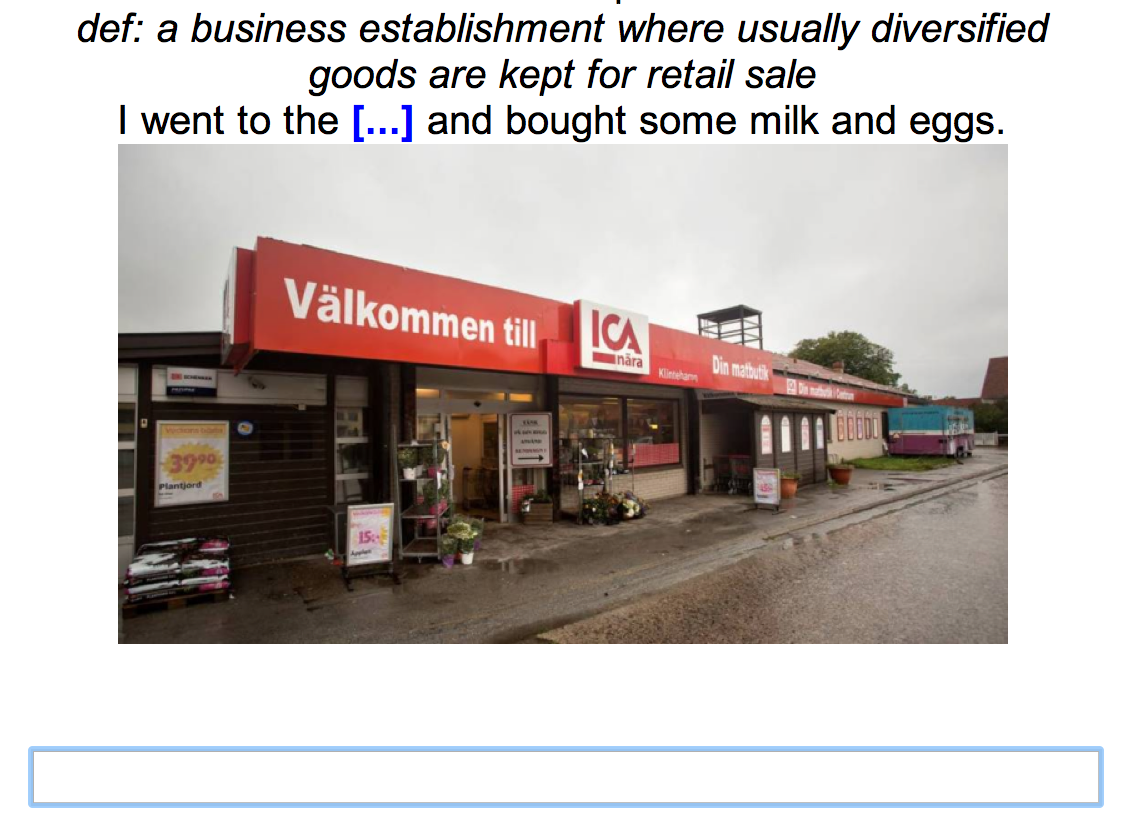
\includegraphics[scale=0.4]{cloze_example.png}
\end{figure}
\end{frame}

%------------------------------------------------
\begin{frame}
\frametitle{Questions}
\begin{itemize}
\item <1-> Can we predict missing word using only the words around it?
\item <2-> What sentences are good example sentences?
    \begin{itemize}
        \item Does length of sentence make a difference?
    \end{itemize}
\item <3-> (If time permits) Where are good sources to find cloze deletion sentences?
\item <4-> Can we use a dictionary to improve performance?
\item <5-> How "good" (words are easy to predict) are dictionary example sentences compared to other sources?
\end{itemize}
\end{frame}


\begin{frame}
\frametitle{Goals}
\begin{itemize}
\item Predict cloze deletion using only the words around it.
    \begin{itemize}
        \item Start without any additional information
        \item See if performance increases using part-of-speech, word sense, etc.
    \end{itemize}
\item Find example sentences with cloze words that are easily predicted.
\begin{itemize}
    \item These sentences would make good flash card sentences when learning a language.
\end{itemize}
\item Compare LSTM with Bidirectional LSTM performance.
\end{itemize}
\end{frame}

%------------------------------------------------

\begin{frame}
\frametitle{Data Sources}
All the data sources I will be looking at are from Göteborgs universitets Språkbanken \cite{spraakbanken}. These datasets all have POS tags, dictionary sense, and various other attributes.
 \begin{itemize}
    \item <1-> Göteborgsposten 2013 - Scrambled sentences from GP articles from 2013.
    \item <1-> 8 Sidor - A news site in easy Swedish.
    \item <1-> A dictionary (also from Språkbanken)
    \item <2> Does the simplified text style in 8 Sidor make for better cloze sentences than GP?
\end{itemize}

\end{frame}

\begin{frame}{Språkbanken Metadata}
    \begin{table}[]
\begin{tabular}{ll}
\hline
Ordattribut (id) & Lokalisering: svenska \\ \hline
word             & ord                   \\
pos              & ordklass              \\
msd              & msd                   \\
lemma            & saknas                \\
lex              & Lemgram               \\
sense            & betydelse             \\
prefix           & förled                \\
suffix           & efterled              \\
compwf           & sammansatta ordformer \\
complemgram      & sammansatta lemgram   \\
ref              & ref                   \\
dephead          & dephead               \\
deprel           & dependensrelation     \\ \hline
\end{tabular}
\end{table}
\end{frame}

\begin{frame}
\frametitle{Machine Learning Approach}
\begin{itemize}
\item Idea is to use a Bidirection LSTM (Neural Network)
    \begin{itemize}
        \item Regular LSTM will use the previous information in a sequence to predict.
        \item Bidirectional LSTM will allow the network to use information from "the future", the end of the sequence. \cite{coursera}
        \item Example: 
        \begin{itemize}
            \item I went to the $\rule{1cm}{0.15mm}$ and bought some milk and eggs.
            \item I went to the $\rule{1cm}{0.15mm}$ and swam 10 laps.
        \end{itemize} 
        \item Both sentence start the same but end very differently, changing the words we would place in the blank.
        \item The hope with using a Bidirection LSTM will be to use the later information with the same weight as previous information.
    \end{itemize}
\end{itemize}
\end{frame}

\begin{frame}
\frametitle{RNN vs BRNN}
\begin{figure}
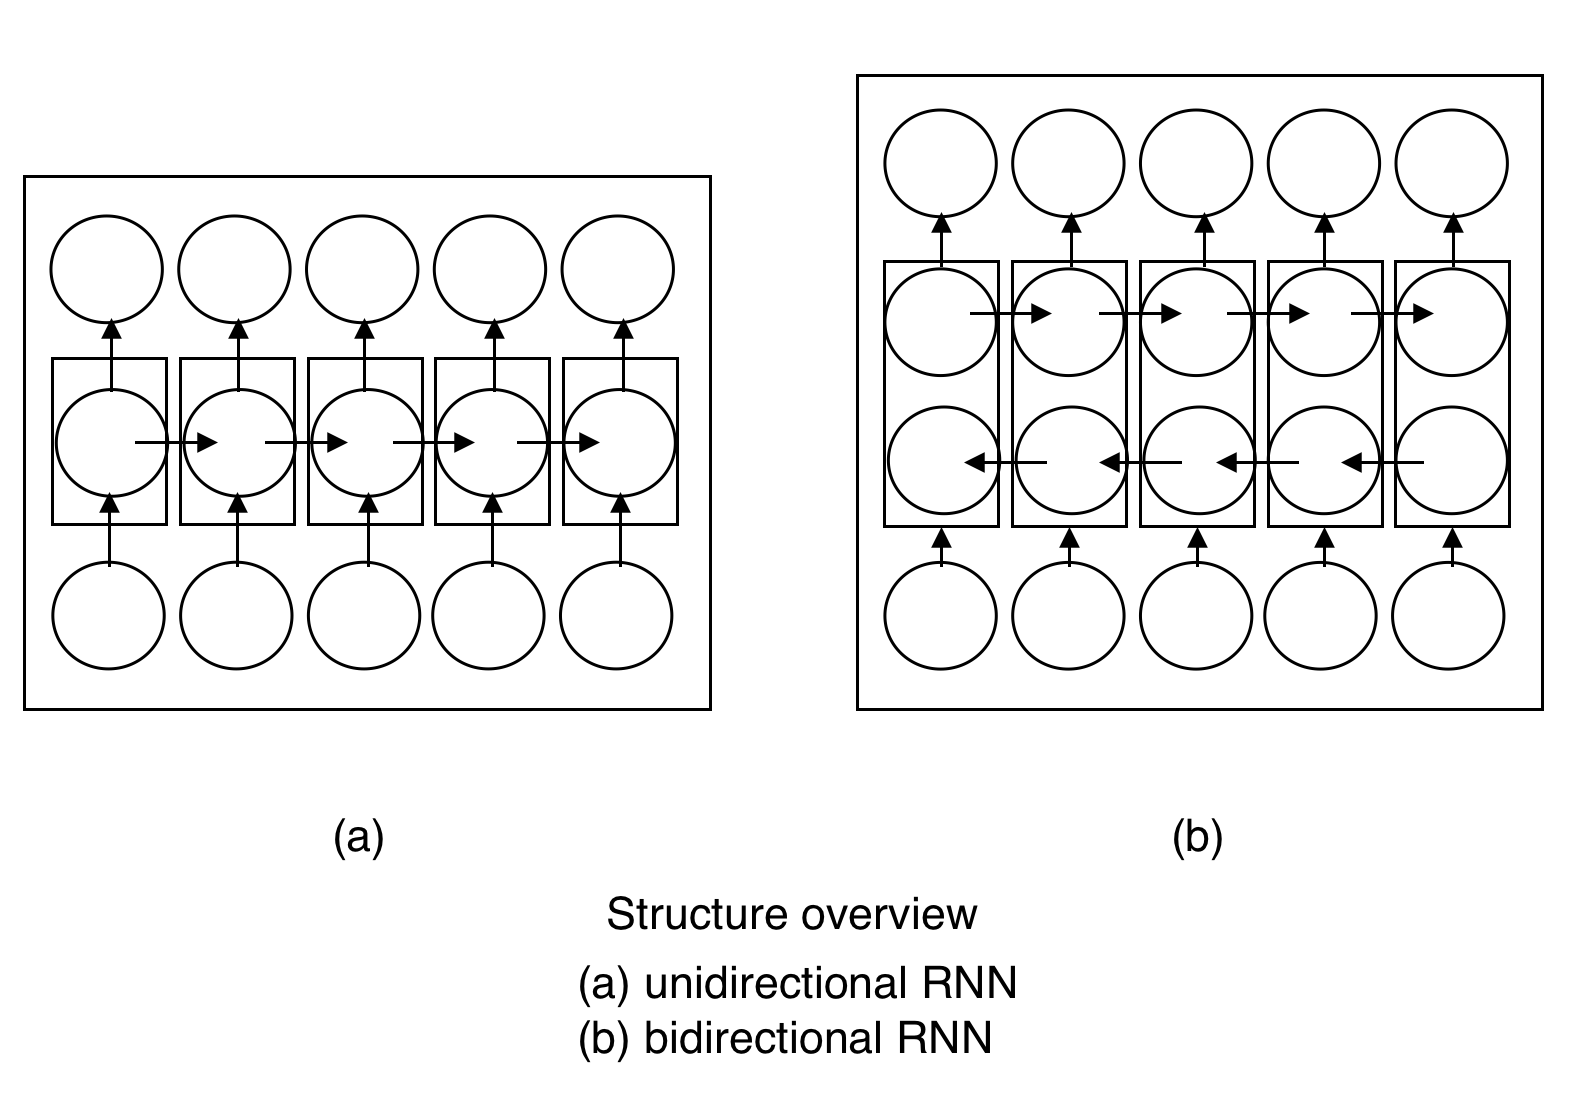
\includegraphics[scale=0.4]{RNN_BRNN.png}
\caption{\cite{blstm}}
\end{figure}
\end{frame}

%------------------------------------------------

\begin{frame}
\frametitle{References}
\footnotesize{
\begin{thebibliography}{1} % Beamer does not support BibTeX so references must be inserted manually as below
	\bibitem{wikipedia}
		Cloze test, 
		\url{https://en.wikipedia.org/wiki/Cloze_test}
		2018
	\bibitem{spraakbanken}
	    Språkbanken, 
		\url{https://spraakbanken.gu.se}
		2018	
    \bibitem{blstm}
    By Incfk8 from Wikimedia Commons
    \url{https://commons.wikimedia.org/wiki/File:RNN_BRNN.png}
    2018
    \bibitem{coursera}
    Sequence Models (Bidirection RNN Video) - Coursera
    \url{https://www.coursera.org/lecture/nlp-sequence-models/bidirectional-rnn-fyXnn}
    2018
    
\end{thebibliography}
}
\end{frame}

%------------------------------------------------

\begin{frame}
\Huge{\centerline{Questions?}}
\end{frame}

%----------------------------------------------------------------------------------------

\end{document}